\chapter{Conclusions \& Further Work}
\label{cha:future_work}
\epigraph{This chapter wraps up this thesis and tries gives some suggestions
  towards eventual future work. It briefly discusses how the developed
  model could be scaled to almost arbitrarily large datasets and how the
  prediction network could be improved with respect to prediction and
  computational performance.
}

\section{Conclusions}%
\label{sec:conclusions}

After a considerable amount of thought was put into the understanding of the
dynamical nature of ESNs and recurrent neural networks in general, I
successfully implemented a framework that is able to predict high-dimensional,
spatio-temporal, chaotic time series.  It can be concluded from the results
chapter, that a general, automated anomaly detection of anomalies in chaotic
systems is possible. The problem of predicting a chaotic system long enough to
detect anomalies was solved without making any assumptions about the underlying
physics.  In addition, the application of the ESN to the prediction problem has
lead to a very cost efficient search algorithm, which is quite striking,
considering that it is able to create said chaotic predictions.

The generality of the prediction framework is another notable point.
The only adjustments that have to be made from one dataset to the next are a
few hyper-parameters.  They can be set approximately by hand by reasoning about
the specific requirements of the given problem.  Both the state size and the
spectral radius of the ESN can be chosen within narrow bounds by examining the
requirements of the problem. The state size should be at least as large as the
period of the examined sequence and the spectral radius must be large enough to
capture its non-linearity.  However, to achieve the best results the exact
choices of hyper-parameters are best left to algorithms such as Bayesian
Optimization.  This reduces the amount of tweaking that has to be done to apply
the model to new datasets to a minimum.

The second goal of finding new physical behaviour in the available climate
model output remains to be achieved. It will require some house keeping in the
analysis part of the code, but all the necessary parts are in place.

With this proof of concept we have shown that the concepts of machine learning
can be of much use in the field of oceanography and climate physics as a whole.
A wider application of the concepts from artificial intelligence and machine
learning promises to make the full potential of climate data exploitable in
completely new ways.



\section{Future Work}%
\label{sec:future_work}

The ultimate goal of this work was to create an algorithm that skims through
huge ocean simulation datasets and returns interesting areas to search for new
physical behaviour. To achieve this, the created anomaly detection, which
can currently process small windows, has to be scaled to work on the large,
global domain. This can be achieved by running many ESNs in parallel over,
possibly overlapping, small windows of the global domain.

Of course, also the current  prediction model can be improved. There is still
much room for improvement by increasing the complexity of the ESN. This would,
most probably, reduce the amount of false positives of the detection.
Additionally, the performance of the ESN could benefit tremendously from
implementing it with a different framework than Tensorflow.

\subsection{Scaling To The Global Domain}%
\label{sub:scaling_to_the_global_domain}

By applying the detection algorithm to small windows of the model output, many
independent ESNs can be run in parallel. This can be scaled until the memory
limitations of the available computing resources are reached.
This spatial parallelization would enable the analysis of the full, global domain.

The parallel ESNs can either operate independently within their window, or the
predictions can be processed into one large super-prediction. For this the
windows must, of course, overlap, which introduces a considerable amount of
communication between the parallel ESN instances into the problem. The
super-prediction can subsequently be divided back into the windows that are fed
back to the individual ESNs. Should physical memory (not STM) become a problem in
the super-prediction approach, the number of individual reservoirs could be
reduced by sharing the large reservoir matrix and only having individual output
weights for each sub-prediction.

The super-prediction approach would also reduce boundary effects like the
large unexpected eddy that entered the Kuroshio prediction window.


\subsection{Predictor Improvements}
With the rather basic setup of a single ESN cell as the prediction network,
there is still much room for improvements of the prediction model itself.  The
most obvious of which would be to add convolutional layers in front of the ESN
cell. This could lead to significant improvements by leveraging the spatial
information of the input as described in
Sec.~\ref{sub:convolutional_neural_nets}.  Unfortunately, this would make the
use of convolutional layers and ain turn an expensive GD algorithm for the
weight optimization necessary, because the convolutional kernels have to be
learned.  By sacrificing the convolutional layer for a standard dense layer the
GD optimization could be avoided, because it is possible to construct untrained
feedforward layers in a similar fashion like the reservoir of the ESN.
Networks that contain untrained feedforward layers are called \emph{extreme
learning machines} and were introduced by [\cite{huang2006}].  The combination
of the two concepts was introduced by [\cite{butcher2013}] and termed
\emph{reservoir with random static projections} (R$^2$SP).  This architecture
promises to solve the memory non-linearity tradeoff by separating non-linear
transformation and internal memory of the network and could thus be much more
powerful.

\begin{figure}
  \centering
  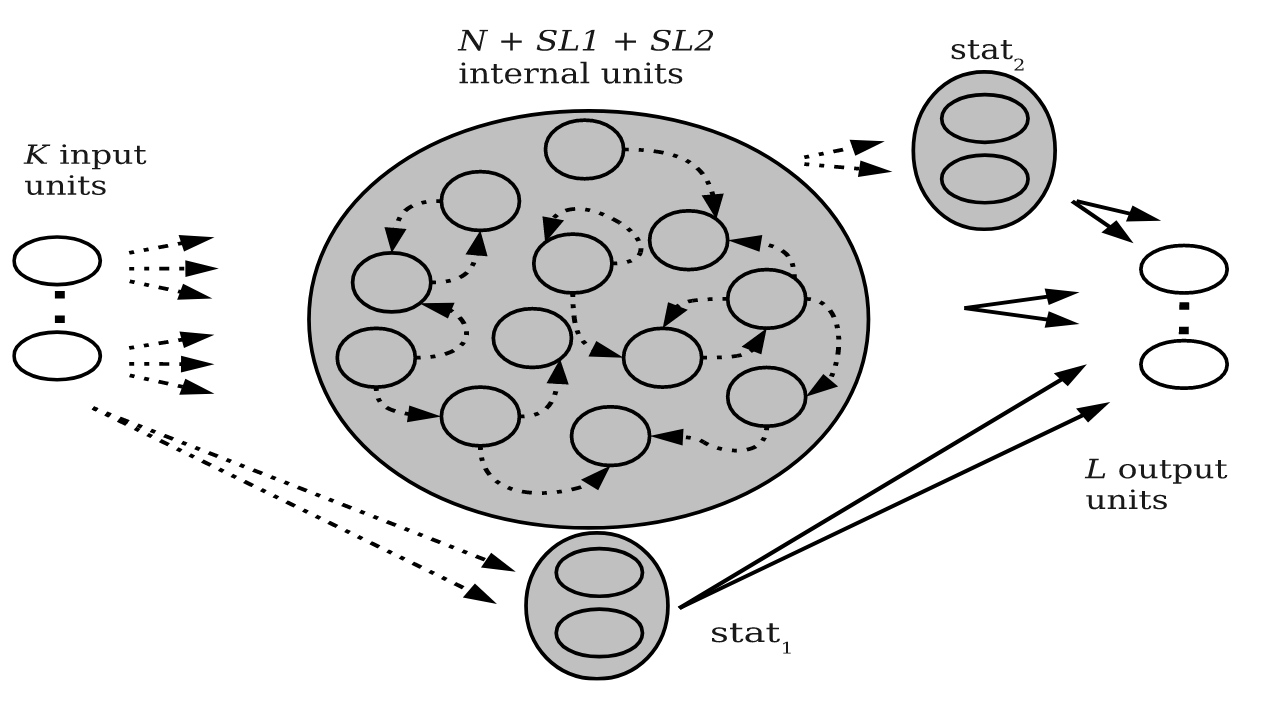
\includegraphics[width=0.6\linewidth]{r2sp.png}
  \caption{Reservoir with random static projections~[\cite{butcher2013}]. The
  stat$_1$ and stat$_2$ layers are static feedforward layers, that take the
  part of the non-linear transformation.  The recurrent internal units
  represent the memory of the network. Their reservoir matrix can be
  initialized with a spectral radius close to one to maximize memory without
  the need of introducing non-linearities.}
  \label{fig:r2sp}
\end{figure}

Another interesting approach to improve the performance of the network would be
to employ \emph{evolutionary optimization} techniques [\cite{fogel1997}] to find
a good reservoir matrix $\wmatr{}$ which could be reused for the whole ocean
dataset.  This would eliminate fluctuations in prediction performance from run
to run.


\subsection{Performance Improvements}
Probably the greatest advantage of the presented approach is its low computational
demand. Creating predictions of a few hundred frames for a window of 30x30
pixels does not take longer than a few seconds on a standard laptop.  However,
for a truly automated application of the model to very large datasets with long
sequences it would be interesting to implement it in another framework.
Tensorflow does not excel in RNN computations and it would be quite simple to
implement the network, for example, in Numpy and parallelize it with Bohrium
[\cite{bohrium}]. This would get rid of a lot of overhead that is caused by the
dynamic graph creation that Tensorflow is doing.

Additionally, the ESN, due to its static nature, holds the potential of being
compiled to an FPGA, which could improve performance even further.


\subsection{Understanding Recurrent Networks}
To date, the general understanding of the ESN and RNNs in general is not very
good.  It is assumed that an RNN classifier needs as many fixed points as it
has features to separate, but fundamental understanding is still lacking.  A
further investigation of the influence of fixed-points and period cycles within
the internal state evolution on the memory and predictive capabilities of RNNs
would be very interesting.  This could lead to a more solid understanding of
how the hyper-parameters of the ESN are influencing its performance.
